\documentclass[a4paper]{article} 
\usepackage{amsmath,amsfonts,amssymb,amsthm}
\usepackage{cite}
\usepackage{algorithmic}
\usepackage{graphicx}
\usepackage{subfigure}
\usepackage{algorithmic}
\setlength{\parindent}{0cm}
\usepackage[left=1.0in, right=1.0in, vmargin=1in]{geometry}

\renewcommand{\algorithmicrequire}{\textbf{Input:}}
\def\ecoli{\emph{E.~coli}}
\def\spades{SPAdes}

\begin{document}
\title{From de Bruijn Graphs to Rectangle Graphs for Genome Assembly}
\footnotetext[1]{Algorithmic Biology Laboratory, St. Petersburg Academic University, St. Petersburg, Russia}
\footnotetext[2]{Dept.\ of Computer Science and Engineering, University of California, San Diego, La Jolla, CA, USA}
\footnotetext[2]{Corresponding authors}
%\footnotetext[3]{These authors contributed equally to this work}
%\footnotetext[5]{St. Petersburg Institute of Informatics of the RAS, St. Petersburg, Russia}
%\footnotetext[5]{Dept.\ of Mathematics, University of California, San Diego, La Jolla, CA, USA}
%\footnotetext[6]{Dept.\ of Computer Science and Engineering, University of South Carolina, Columbia, SC, USA}
\footnotetext[4]{This work was supported by grants from the National Institutes of Health, USA (NIH grant 3P41RR024851-02S1)
and the Government of the Russian Federation (grant 11.G34.31.0018).}

%\author[Pham et al.]{Son K. Pham\textsuperscript{1,3}
%	\and Dmitry Antipov\textsuperscript{4,3}
%	\and Alexander Sirotkin\textsuperscript{4}
%	\and Glenn Tesler\textsuperscript{5}
%	\and Pavel A. Pevzner\textsuperscript{4,1}
%	\and Max A. Alekseyev\textsuperscript{2,4,6,7}
%}


\author{Nikolay Vyahhi\textsuperscript{1}, Son Pham\textsuperscript{2} and Pavel Pevzner\textsuperscript{2}}
\date{\today}
\maketitle

\abstract{The jigsaw puzzles were originally created by painting a picture on a 
rectangular piece of wood, and further cutting it  into
smaller pieces with a jigsaw.
The objective of the Jigsaw Puzzle Problem  is to find an arragement of these pieces  that (i) fills up the rectangle, and (ii) 
neighboring pieces have ``matching'' boundaries with respect to color
and texture.
While a general Jigsaw Puzzle Problem is NP-complete~\cite{Demaine07}, we introduce its simpler version  (called {\em Rectangular Puzzle Problem}) and
study the {\em  rectangle graphs}  for assembling such puzzles.  
While previous  applications of the jigsaw puzzle problem were  limited to 
the assembly and repair of broken objects or 
the archeological restoration, Bankevich et al, 2012~\cite{Bankevich12} recently demonstrated  that the Rectangular Puzzle Problem 
models the problem of assemblying genomes from paired reads.  This model differs from the traditional model for genome assembly (assembling 1-dimensional overlapping puzzle) and presents some new algorithmic challenges that haven't been addressed in \cite{Bankevich12}. 
We demonstrate that addressing these challenges improves on results in \cite{Bankevich12} and  other existing assembly algorithms in the case of bacterial genomes (including particularly dfficult case of genome  assemblies from single cells). 
}

\newpage
\section{Introduction}

%{\tt Add affiliations} 

%{\tt The paper requires A LOT of work - it is nowhere close to submission. I believe my revision significantly simplifies and shortens the presentation. 

%The current version makes an emphasis on "explaining" the Bankevich et al., 2012 in a new language and makes it easier to digest using an analogy.
% However, it talks very little about the challenges addressed by Kolya that we discussed.
% If we have only 2 paragraphs describing these challenges, what has been done to implement rectngles
% and why it could not have been done in a week? I believe there were challenges but they are not adequately addressed in the paper.

%Kolya, can you address why the coverage was dropped as compared to the standard version of SPAdes and reflect it in the paper? 

%WHAT IS THE PLAN FOR THE REMAINING 2.5 DAYS? 



The recent proliferation of next generation sequencing has enabled 
new experimental opportunities and, at the same time, 
raised formidable computational challenges. 
When the length of a repeat in the genome exceeds the read length, it becomes difficult to
 ``match'' the flanking regions of this repeat in the assembly.  To alleviate this
problem, sequencing technologies were extended to produce {\em read-pairs},  
pairs of reads separated by an estimated insert length. 
 Because insert sizes are longer than the read length, read
pairs span longer repeats and could potentially match the regions
flanking a repeat as long as it is longer than the insert length. Chaisson et al., 2009~\cite{Chaisson09} even 
argued that ``read length does not matter'', i.e., that assembling genome from read-pairs  
is nearly equivalent to assembling genome from long virtual reads (with length equal to the insert length).
However, implementing this idea in practice faces some algorithmic challenges since until recently there were 
no elegant algorithmic models for effective utilization of {\em all information} provided by read-pairs.  

While assembling single reads can be elegantly modelled by 
{\em de Bruijn graphs}~\cite{Idury95 ,Pevzner01}, applications of 
the de Bruijn graphs to assembling read-pairs remains a challenge. 
This  challenge  was first addressed by \cite{Pevzner01b} and similar ideas were incorporated to other assemblies.  Pevzner and Tang, 2001~\cite{Pevzner01b} first constructed the de Bruijn
graph and further checked for a path between the two reads within a read-pair consistent with the constraints imposed by the
insert size. If only one such path exists, a {\em read-pair transformation}
could be applied to  transform a read-pair into a long {\em virtual} path.  Essentially, this amounted
to transforming a read-pair into  a virtual  read where the gap between the
reads is filled in with the nucleotide sequence representing the found path. %(potentially matching the surrounding regions of a repeat).  

While this and similar methods~\cite{Zerbino09, Butler08, Boisvert10, SOAP,Simpson09,Peng10} 
had a large impact on genome assembly,  they fail in complex repeat-rich
regions, where there are multiple paths between the reads within read-pairs. Recently,~\cite{Medvedev11} introduced
paired de Bruijn graph that directly incorporates mate-pair into the graph structure and bypasses the problem of multiple
paths in the previous approaches. However, paired de Bruijn graph were introduced as a theoretical framework and mainly aimed 
at the unrealistic case when {\em precise and fixed} distances between reads are known. 
%Paired de Bruijn Graph faces difficulty on real dataset where 
%the distances between reads within read-pairs varies. 
 To address this bottleneck,  Bankevich et al., 2012 recently  introduced the  {\em rectangle graph} by  generalizing the problem of a string 
reconstruction from its paired substrings to a variation of the jigsaw puzzle problem. 

%    De Bruijn graphs have been used in many areas of bioinformatics, including genome assembly~\cite{Pevzner01},
%    repeats classification~\cite{Raphael04}, protein sequencing~\cite{Bandeira07},
%    and synteny blocks identification~\cite{Pham10}. In these applications, de Bruijn graphs are either constructed from a string or from a set of sub-strings of an
%    unknown string via gluing rules~\cite{Pham10,Raphael04}. 
%    In this work, we show that the idea of gluing rules for strings in de Bruijn graph can be
%    also adopted for multiple non-string objects, which can be used for the reconstruction of an object from
%    its broken pieces --- a general abstraction of the jigsaw puzzles. 


The jigsaw puzzles were originally created by painting a picture on a rectangular piece of wood
and cutting it into
small pieces with a jigsaw. The jigsaw puzzles assembly amounts to  arranging these small pieces into a ``valid'' picture with no gap or overlap between
them. 
%Formally, the jigsaw problem can be defined as follow. Given a set $SP = \{ P_0, P_1,\ldots, P_n\}$ where $P_i$ %represents the $i^{th}$ piece.
%The objective of any jigsaw puzzles is the rearragement of these pieces into a single structure with no gaps left %between adjacent pieces. Additionally,
%neighboring pieces must share an identical boundary as well as having similar color and 
%texture near the boundary.
Previous  algorithmic studies of the jigsaw puzzle problem considered the problems of  assembly and repair of broken objects~\cite{Uccoluk99} 
or the restoration of archaeological findings~\cite{Kampel04}. Here we show
that the assembly problem from paired reads can also be formulated as a simple version of the jigsaw puzzle problem. 
In particular, in section 2, we describe a simple version of jigsaw puzzle problem (called rectangle puzzle problem) and define the rectangle graphs to solve this 
problem. In section 3 we show the relation between the rectangle puzzle problem and  genome assembly from read-pairs. In section 4, we describe how to adapt our approach 
to work with inexact insert size. In Section 5 we apply the rectangle graphs to bacterial genome assembly.  

We empasize that previous assembly approaches modeled the  problem as a 1-dimensional  
jigsaw puzzle with {\em overlapping} pieces~\cite{Jones04}.  
In contrast, the rectangle graph model assembly as traditional jigsaw puzzle with non-overlapping pieces. Our analysis extends the analysis in Bankevich et al., 2012~\cite{Bankevich12} to real challenges encountered in applications of rectangle graphs and presents the rectangle graph concept in a more intuitive way.

\section{Rectangle Puzzle Problem} 

Consider $n+1$ points $x_0=0 < x_1 <  \ldots < x_n$ on $x$-axis and $m+1$ points $y_0=0 < y_1 <  \ldots < y_m$ on $y$-axis. Points $(x_i,y_j)$ form a 2-dimensional grid consisting of $n \cdot m$ small rectangles filling up the grid with corners $(0,0), (0,y_m), (x_n,0)$ and $(x_n,y_m)$. By analogy with the puzzle assembly we assume that the grid is ``painted'' and the goal is to assemble small rectangles into the painted grid in such a way that rectangles fully fill up the grid and that the colors at the sides of of neighboring  rectangles match. 

Consider a continuous non-self-intersecting curve from $(0,0)$ to $(x_n,y_m)$ in the grid that crosses  
the sides of the rectangles at points $p_0=(0,0), p_1, \ldots , p_N=(x_n,y_m)$ (in their order along the curve). The curve is called {\em traversing} if $p_i$ and $p_{i+1}$ belong to different sides of a rectangle (for $0 \leq i \leq N-1)$ and if there are exactly two red points on the sides of each rectangle. For simplicity we assume that the direction of the traversing curve (from $(0,0)$ to $(x_n,y_m)$) within each rectangle is known and that the curve does not pass through the corners of the rectangles except for points $p_0=(0,0)$ and $p_N=(x_n,y_m)$.  


In the {\em rectangle puzzle}  problem we assume that red points in the grid form a traversing curve and the goal is to assemble the grid from (painted) rectangles. 
More precisely, we want to generate all possible assemblies of the rectangles into the grid that respect the painting (See Fig.~\ref{fig:curve}a). 
It appears to be a trivial problem in the case of Fig.~\ref{fig:curve}a where the painting has enough details to unambiguously reveal all rectangles that share sides. 
However, it becomes less trivial in the case of Fig.~\ref{fig:curve}b with only white and red colors. 
{\tt It would be great to design Fig.2b in such a way that there exist ambiguities and illustrate them further in the construction of the rectangle graph.} 

 
\begin{figure}
\begin{center}
	\begin{tabular}{l@{\extracolsep{13pt}}l}
		(a) & (b) \\
		\vtop{\vskip0pt\hbox to.45\textwidth{\includegraphics[width=.45\textwidth] {fig/gridGraphCurvePicture.eps}}}
		&
		\vtop{\vskip0pt\hbox to.45\textwidth{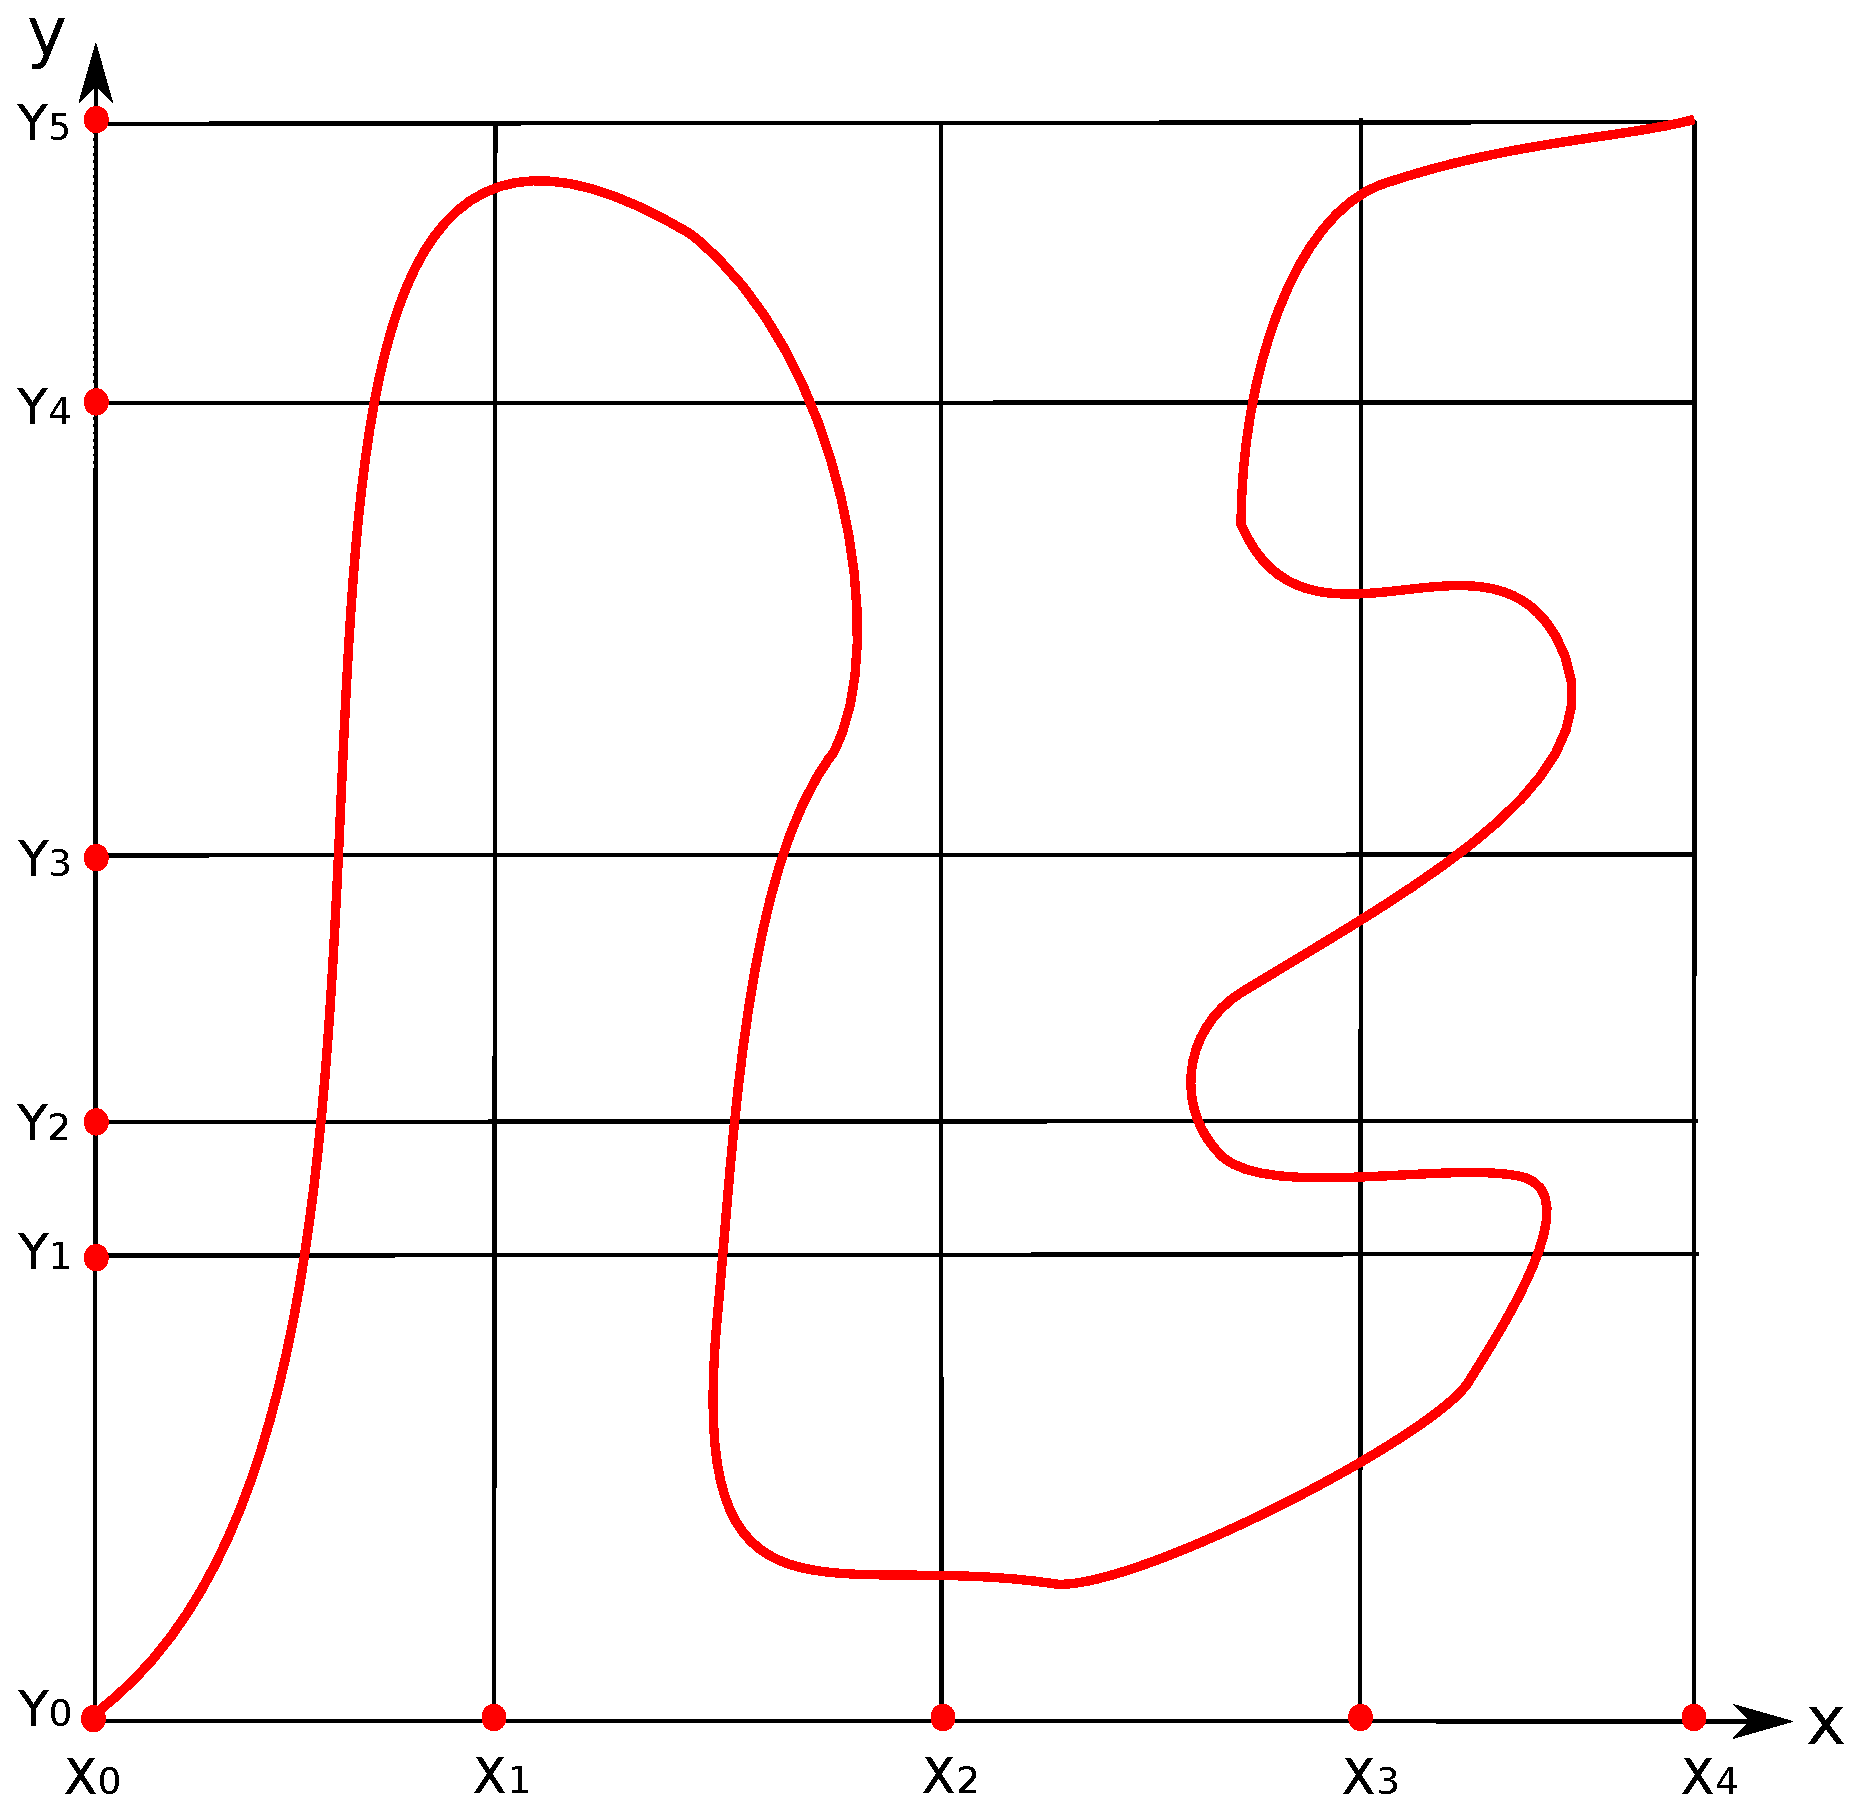
\includegraphics[width=.45\textwidth] {fig/gridGraphCurve.eps}}}
	\end{tabular}
\caption{Rectangular Puzzle Problem. (a) Points $x_0, \ldots ,x_4$ and $y_0, \ldots ,y_5$  (red points) form a 
rectangular grid consisting of $4\times 5$ rectangles. 
The traversing curve in the grid is shown in red. (b) Picture is removed.{\tt Describe (a) and (b)}}
\label{fig:curve}
\end{center}
\end{figure}
 
\begin{figure}
\begin{center}
	\begin{tabular}{l@{\extracolsep{13pt}}l}
		(a) & (b) \\
		\vtop{\vskip0pt\hbox to.45\textwidth{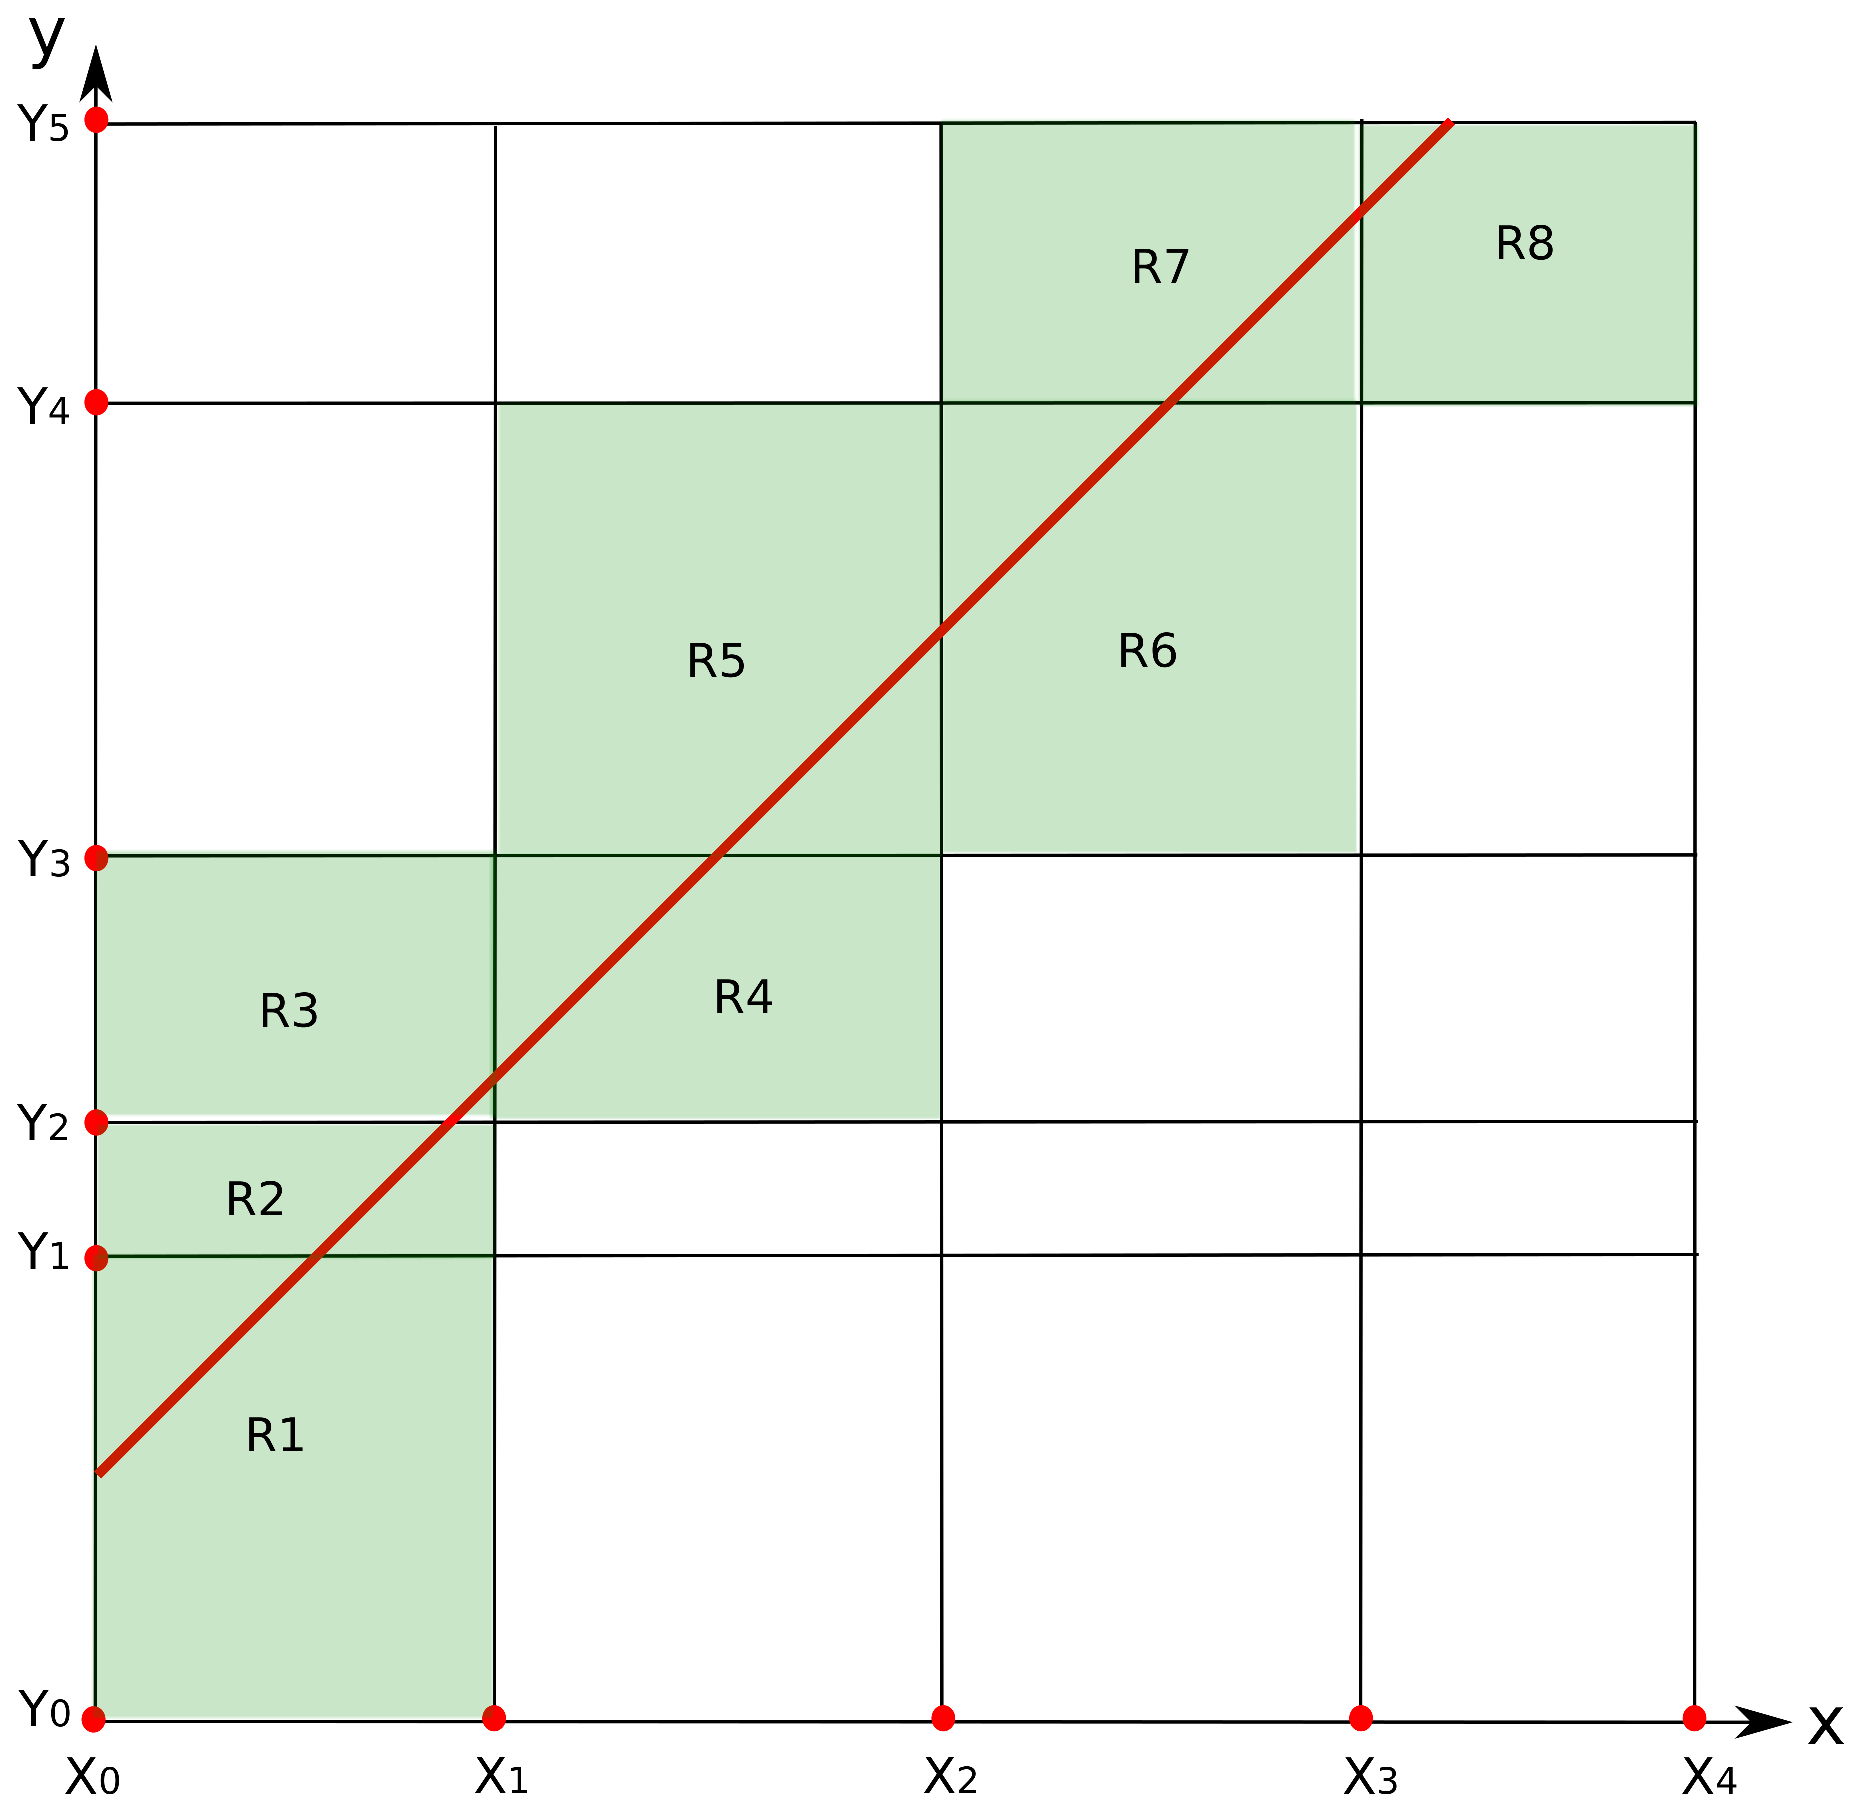
\includegraphics[width=.45\textwidth] {fig/gridGraphLine.eps}}}
		&
		\vtop{\vskip0pt\hbox to.45\textwidth{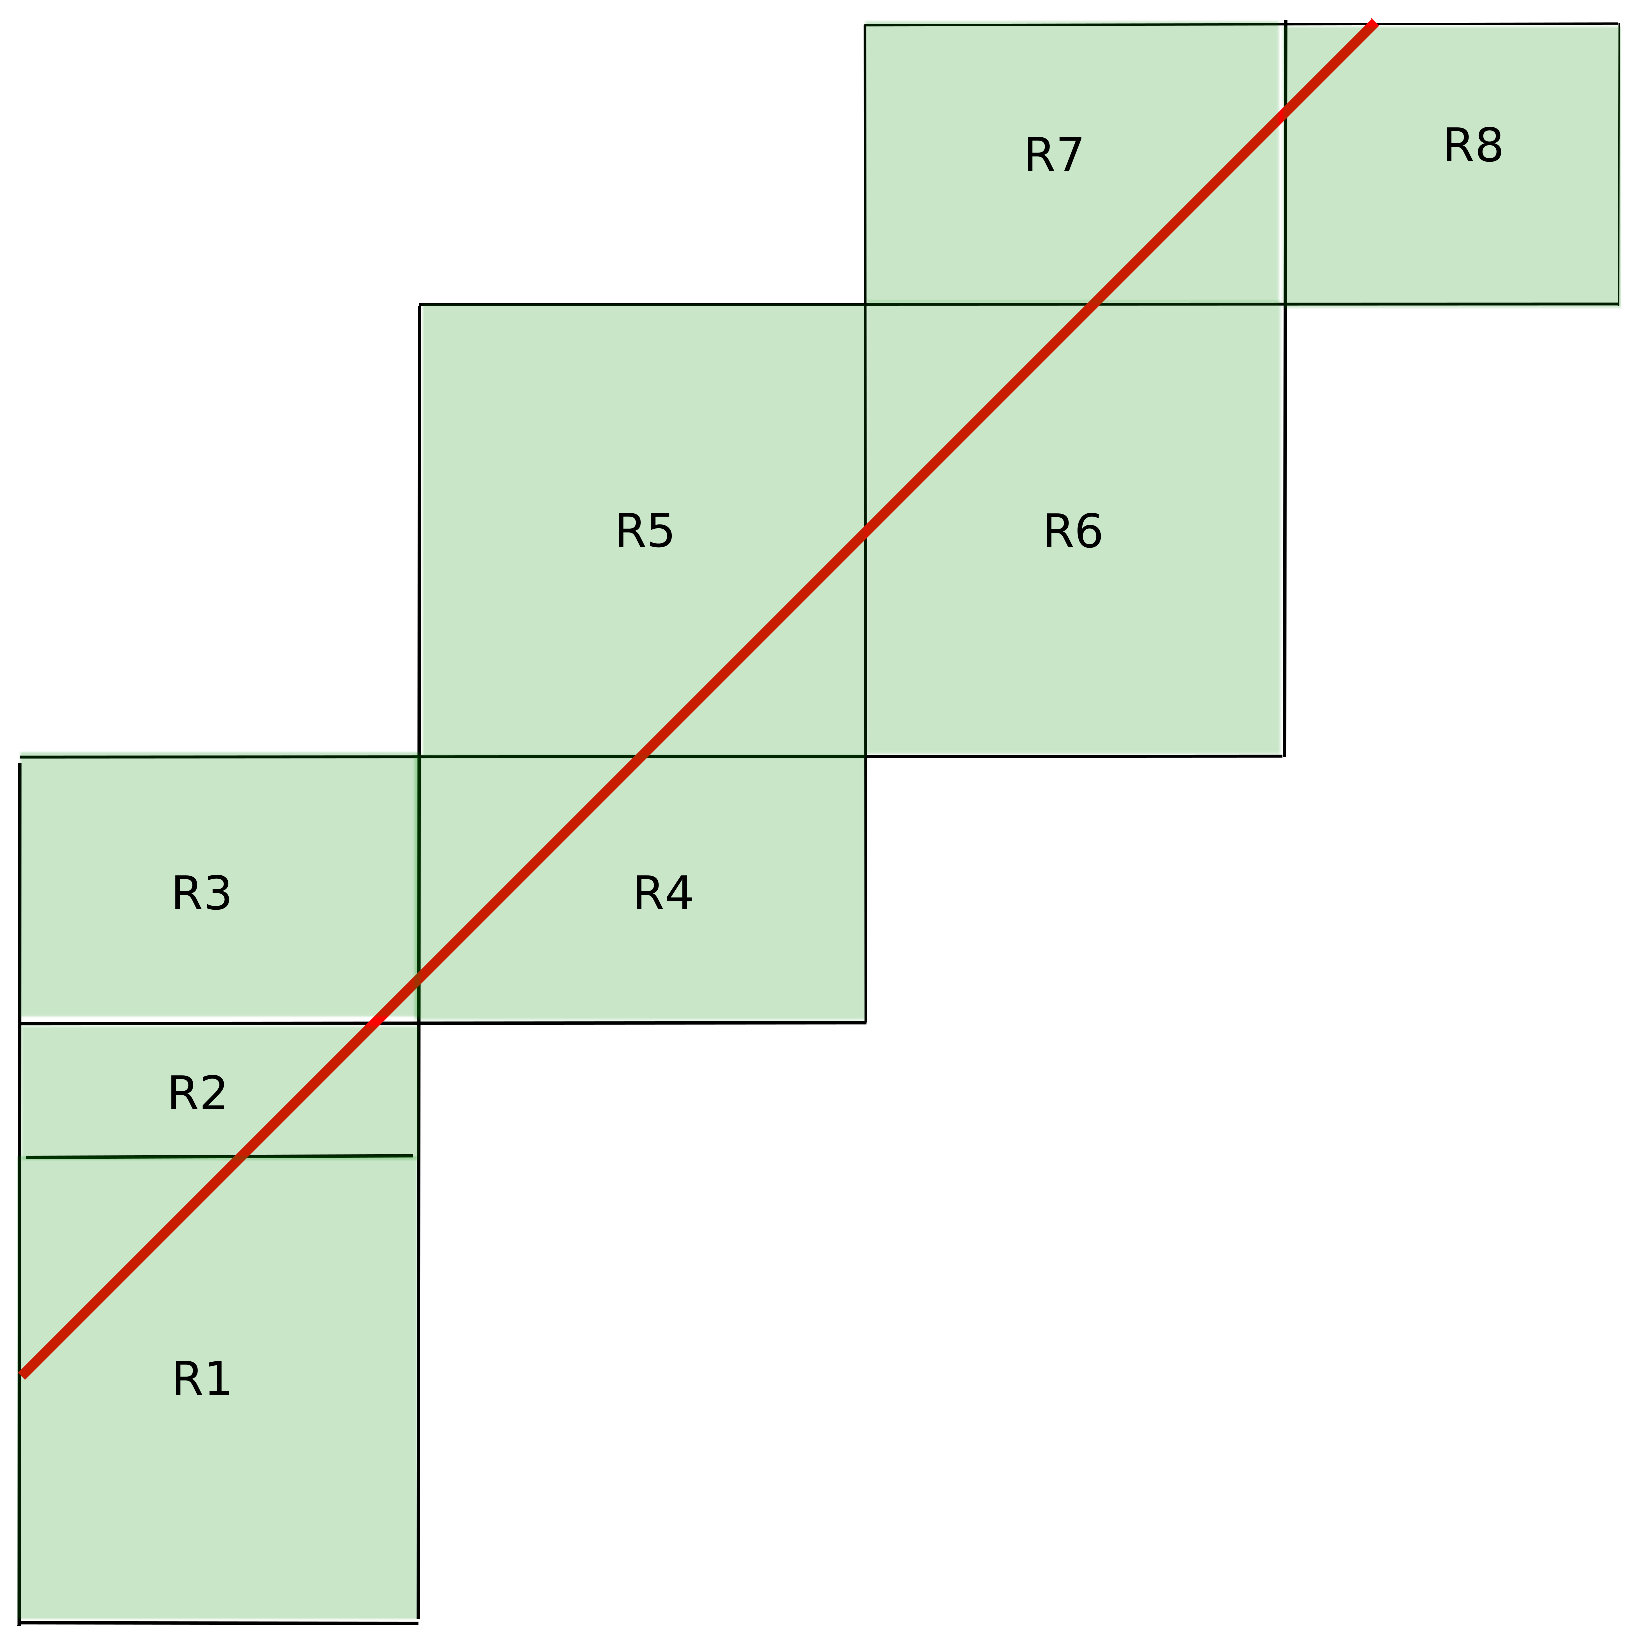
\includegraphics[width=.45\textwidth] {fig/gridGraphLineSimple.eps}}}
	\end{tabular}
\caption{TODO: Describe (a), (b) and refer it}
\label{fig:line}
\end{center}
\end{figure}

%:{\tt Decide on the color. In the text the curve is called red but in the figure it is blue.} 

The red curve enters and leaves each rectangle $R$ through sides that we call $source(R)$  and $sink(R)$ correspondingly.  Since points $p_0=(0,0)$ and $p_N=(x_n,y_m)$ belong to two sides of the bottom-left and upper-right rectangles, correspondingly, we will arbitrarily assign them to the horizontal sides of these rectangles to avoid ambiguities. 
We assume that every side $S$ of a rectangle is assigned a label $label(S)$ (that encodes the painting of this side) and that differently painted sides are assigned different labels.  We represent a rectangle $R$ by a directed edge $edge(R)$ from vertex $label(source(R))$ to vertex $label(sink(R))$.  For convinience, we assign identical and unique labels to the sides of rectangles containing the first and the last points ($(0,0)$ and $(x_n,y_m)$ on the red curve. 

Below we describe the rectangle graph that allows one to generate all solutions of the rectangle puzzle problem. 

\textbf{Rectangle Graph:}
\begin{itemize}
\item  Define a graph $G$ with $n \cdot m$ edges and $2 \cdot n \cdot m$ vertices by introducing an edge $edge(R)$ for each rectangle $R$. 
\item The rectangle graph is formed by gluing identically labelled vertices of $G$.
\end{itemize}
One can notice that the rectangle graph is simply the de Bruijn graph on strings of length 2 in the alphabet of all labels. Each rectangle assembly corresponds to an Eulerian  cycle in this graph (we remind the reader that starting and ending points in the traversing curve were glued into the same vertex in the rectangle graph.) 
All 
Eulerian cycles  can be efficiently generated using the BEST \cite{best} theorem thus reducing the rectangle puzzle
assembly to enumerating Eulerian cycles in the rectangle graph, a well studied problem \cite{abrham80}. 
However, not every Eulerian cycle corresponds to a valid solution of the rectangle puzzle since some solution may force rectangles to overlap or may correspond to assemblies that do not form a rectangular grid. However, it is easy to check if a given Eulerian cycle corresponds to a valid rectangle assembly in linear time. 

Below we limit attention to traversing {\em lines} (rather than {\em curves})   and  relax the condition for the traversing curve (line) to visit  {\em all} rectangles: 
\begin{itemize} 
\item We relax the condition for the traversing curve to visit {\em all} rectangles.  In this case we are only interested in assembling  rectangles into a {\em subgrid}  formed by rectangles with red points (rather than assembly of all rectangles into the full grid). 
\item The traversing curve is a line $y=x+D$ that does not necessarily starts at $(0,0)$ and ends at $(x_n,y_m)$. In this case, every Eulerian cycle corresponds to a valid subgrid assembly and thus no additional checks are needed to verify that the assembly (given by an Eulerain cycle) is valid. 
\end{itemize}

Below we continue using the term the ``rectangle puzzle'' while referring to the case of \emph{traversing lines} that do not visit all rectangles. 

\section{Generating Rectangle Puzzle from Genome}


We represent a genome $a_1 \ldots a_N$ as a circular string over the alphabet of nucleotides $\{A,T,C,G\}$. 
Below we fix $k$ and use an alternative representation of the genome in the alphabet of all $(k-1)$-mers (a $k$-mer is a string of length $k$). In this representation,  $Genome=g_1 \ldots g_N$, where $g_i$ is a $(k-1)$-mer $a_i \ldots a_{i+k-2}$ starting at the $i$-th positon of the genome.  


Given a $k$-mer $s = s_1\ldots s_k$,
we define $prefix(s)= s_1\ldots s_{k-1}$ and $suffix(s) = s_2\ldots s_k$. Given a multiset of all $k$-mers  from $Genome$, 
the (standard) de Bruijn graph $DB(Genome,k)$ has directed edge $(prefix(s),suffix(s))$
for each $k$-mer $s$ in $Genome$.  The genome defines an Eulerian cycle in its de Bruijn graph. 

A vertex $v$  in a graph precedes (follows) vertex $w$ if there exists an edge from $v$ to $w$ (from $w$ to $v$). The indegree (outdegree)  of a vertex 
is the number of vertices preceding (following) it.  A vertex is called a branching vertex if either its indegree or its outdegree is larger than 1. A path in a graph is called a {\em non-branching path}  if all vertices in this path (with exception of the the first and the last ones) have indegree and outdegree
both equal to 1. 

The de Bruijn graph $DB(Genome,k)$ partitions $(k-1)$-mers from the $Genome$ into branching (if they correspond to branching vertex in $DB(Genome,k)$ and non-branching. Similarly, all 
positions of $Genome$ are partitioned into branching (if a $(k-1)$-mer  starting at this position is branching) and non-branching. For simplicity, we assume that the circular genome ``starts'' at a branching position 0 and ends at the branching position $N$ (since the genome is circular, these two positions represent the same site in the genome and the same vertex in the de Bruijn graph).  

We denote the branching positions in $Genome$ as $x_0=0 < x_1 < \ldots x_n=N$.  
Given an integer $d$, we define the rectange puzzle $Puzzle(Genome,k,d)$ as follows. The grid consisting of $n \cdot n$ rectangles is defined by points $x_0=0 < x_1 < \ldots <x_n=N$ on $x$ axis and the same list of points on $y$-axis. The red line is defined by the equation $y=x+d$.  The ``paint'' (label) at position $(x,y)$ of the grid is defined as $(label(x),label(y),color)$ where $label(x)$ and  $label(y)$ are 
$(k-1)$-mers starting at position $x$ and $y$ in $Genome$, and $color$  
is ``red'' or ``white'' depending on whether $(x,y)$ is located on red line or not. 
The label of the side of a rectangle is defined as an ordered list of all labels of (integer) points located on this side. 

\section{Generating Rectangle Puzzle from Read-Pairs (Exact Distance Between Reads)}

While in the real assembly problem, the genome is unknown and only read-pairs are available, we show below how to generate an instance of the rectangle puzzle problem from read-pairs. 

 Given a set of read-pairs, one can construct the de Bruijn graph from reads and thus generate a list of branching vertices in this graph. Every pair of non-branching paths in the de Bruijn graph define a rectangle and labeling of all its (integer) points.  

When the distance between reads within read-pairs {\em equal} to $d$ (for all read-pairs), one can find $(k-1)$-mers in $Genome$ separated by distance exactly $d$ and thus reconstruct how the the red line crosses the rectangles in the rectangle puzzle (see Bankevich et al., 2012 for details).  Some complications are possible when two non-branching paths  in the de Bruijn graph give rise to multiple rectangles (repeats in genome), e.g., some of them crossed by the red line while others are not. In this case, two non-branching paths give rise to multiple {\em types} of equally-sized rectangles that vary in whether and how the red line crosses them.  For the sake of simplicity, we will assume that we are able to derive the multiplicity of  each type of such rectangles.\footnote{Coverage of the pair of non-branching paths by paired reads allows one to estimate the multiplicity of each type, at least for standard (multicell) a
ssembly.}  See below on how to address this and other complications that were not covered in \cite{Bankevich12}. 

\section{A Simple Jigsaw Problem}

We consider a two-dimensional rectangular jigsaw puzzle created by the following procedure:
In stead of a complicated picture as it is usually the case for jigsaw puzzles, we simply draw a line $(d): y = x + D$ on a 2-$d$ coordinate Oxy.
On the vertical axis, define $n$ points: $A_1$, $A_2$, \ldots, $A_n$; on the horizontal axis, define $m$ points
$B_1, B_2, \ldots, B_m$. The $m\times n$ combinations of these points defines a grid with $m\times n$ rectangles.  We further assign a label for each edge (there are
$m\times n$ edges) of the grid. The labeling of these edges is not unique, i.e., there may be different edges with the same label. 
%We limit our attention to the
%part of the grid that is intersected by the line and ignore all other parts (rectangles) that are not.
Given a fixed value $D$,  the line $(d): y = x + D$ defines the \emph{diagonal grid graph} by retaining only the rectangles that are intersected by $(d)$.
Similar to the assembly problem where one attempts to reconstruct the genome from its
substrings, here we want to reconstruct the diagonal grid graph from individual rectangles.
In the classical sequence assembly problem, a fragment of the sequence is a substring. In this context, a \emph{fragment} is a
rectangle in the grid graph with a fragment of the line $(d)$ on it. 
An intuitive approach is to put the rectangles together such that their boundaries and diagonal lines match~\footnote{
For simplicity, we define the direction of each rectangle so that its orientation
is uniquely define in 2D space}. Below, we formally define what constitutes
a valid solution for our simplified jigsaw version.

Given $n$ rectangles, each with a directed fragment of the line (d). For a rectangle $R$, we denote In(R): 
    the starting point of the fragment and Out(R): the ending point of
the fragment. The edges containing In(R) and Out(R) are called incoming face and outgoing face correspondingly. When In(R)/Out(R) coinsides with the
angle points of the rectangle, the face becomes a single point.
Rectangle $R_1$ and $R_2$ are called neighbours if they share at least one vertex. Given two neighbouring rectangles $A$ and $B$, $A$ is
called extendable by $B$ ( or $B$ extends $A$) if the incoming face of $B$ and the outgoing face of $A$ as well as the locations of
the incoming and outgoing points are exactly aligned. Fig.~\ref{fig:basic} lists all 3 possible extensions of a given rectangle.
A figure is a valid solution to the jigsaw problem if every rectangle has one neighbor that extends it.
It is clear from the definition of the extension of pieces that a single line will be assembled from its fragments on separated rectangles.
We are interested in the following problem.
\begin{figure}
\begin{center}
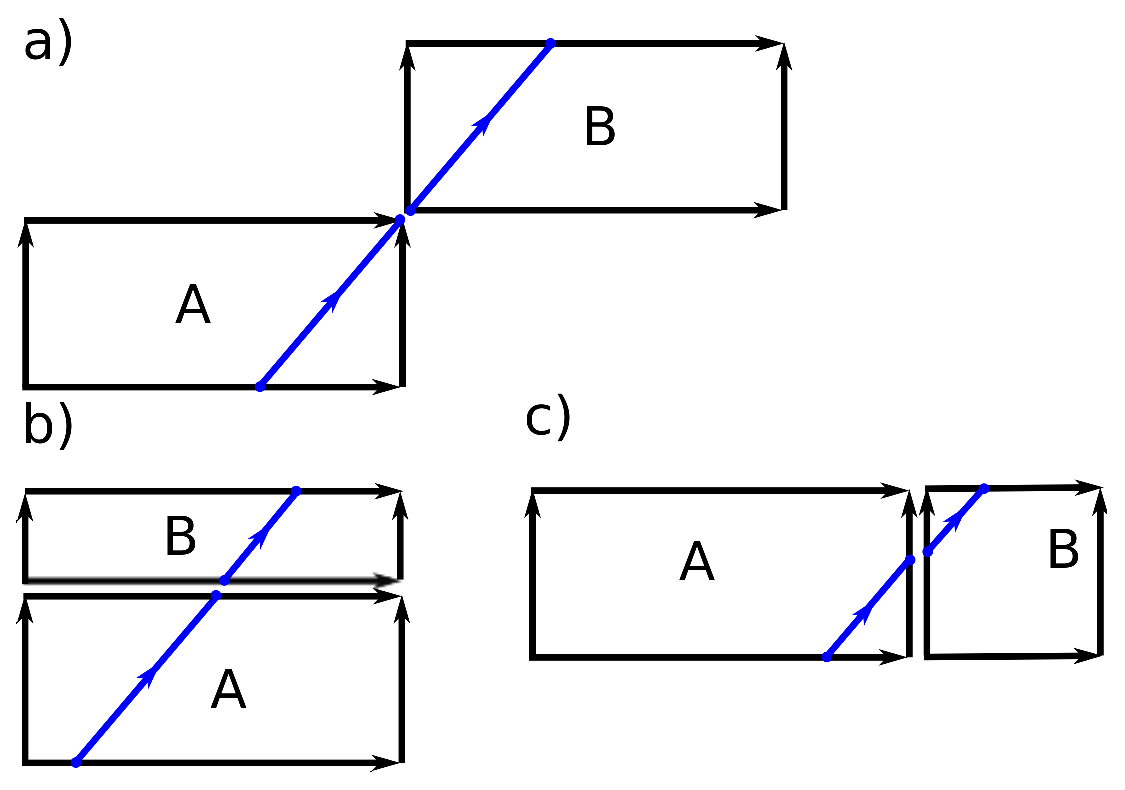
\includegraphics[scale=0.3]{fig/basic.eps}
\end{center}
\label{fig:basic}
\caption{Three possible extensions of rectangle $A$ based on its outgoing face.}
\end{figure}

\textbf{Line Assemblying Puzzle}: \emph{Given $n$ rectangles generated by the described jigsaw generation procedure}
\begin{itemize}
\item \emph{Find the number of valid solutions.}
\item \emph{Enumerate all possible valid solutions.}
\end{itemize}

Below we define the rectangle graph which directly leads to the solution of this problem.

\textbf{Rectangle Graph:}
\begin{itemize}
\item  Define an initial graph $G_0$ on $2n$ vertices. For each rectangle $R$, introduce two new vertices $u$, $v$ and form an edge $u \rightarrow v$.
Label $u$ by the incomming face and the position of IN(R) in the face.
% If this position == 0 or == end_of_edge, then we label with vertex. So label can be only: (vertex, (edge, position)) or ((edge, position), vertex) or (vertex, vertex). This three correspond to tree type of gluing from Figure 1.
Label $v$ by the outgoing face and the position of OUT(R) 
in the face.
\item Glue vertices of $G_0$ together if they have the same label.
\end{itemize}

It is clear that each Eulerian tour in the rectangle graph corresponds to a valid solution of the jigsaw puzzle. The number of solutions is the number of
Eulerian tours in the graph, which can be characterized by the BEST \cite{best} theorem. The problem of enumerating all valid figures is reduced to the problem of enumerating
all Eulerian tours in the rectangle graph, a well studied problem \cite{abrham80}. 
Note that the original figure also corresponds to an Eulerian tour in this graph.  

%    \subsection{A General Fragment Assembly Problem}
%    A general fragment assembly problem tends to reconstruct the original \textbf{object} from its fragments. In particular, sequence fragment assembly tends to
%    reconstruct the original string from its substrings. Similarly, we can define the diagonal grid graph assembly problem from the set of all its rectangles. In particular,
%    given a set of rectangles, one approach to reconstruct the original diagonal grid graph is to align these fragments together such that the edges of adjacent rectangles
%    share the same label and the diagonal line can continue from one rectangle to its adjacent one.



\begin{figure}
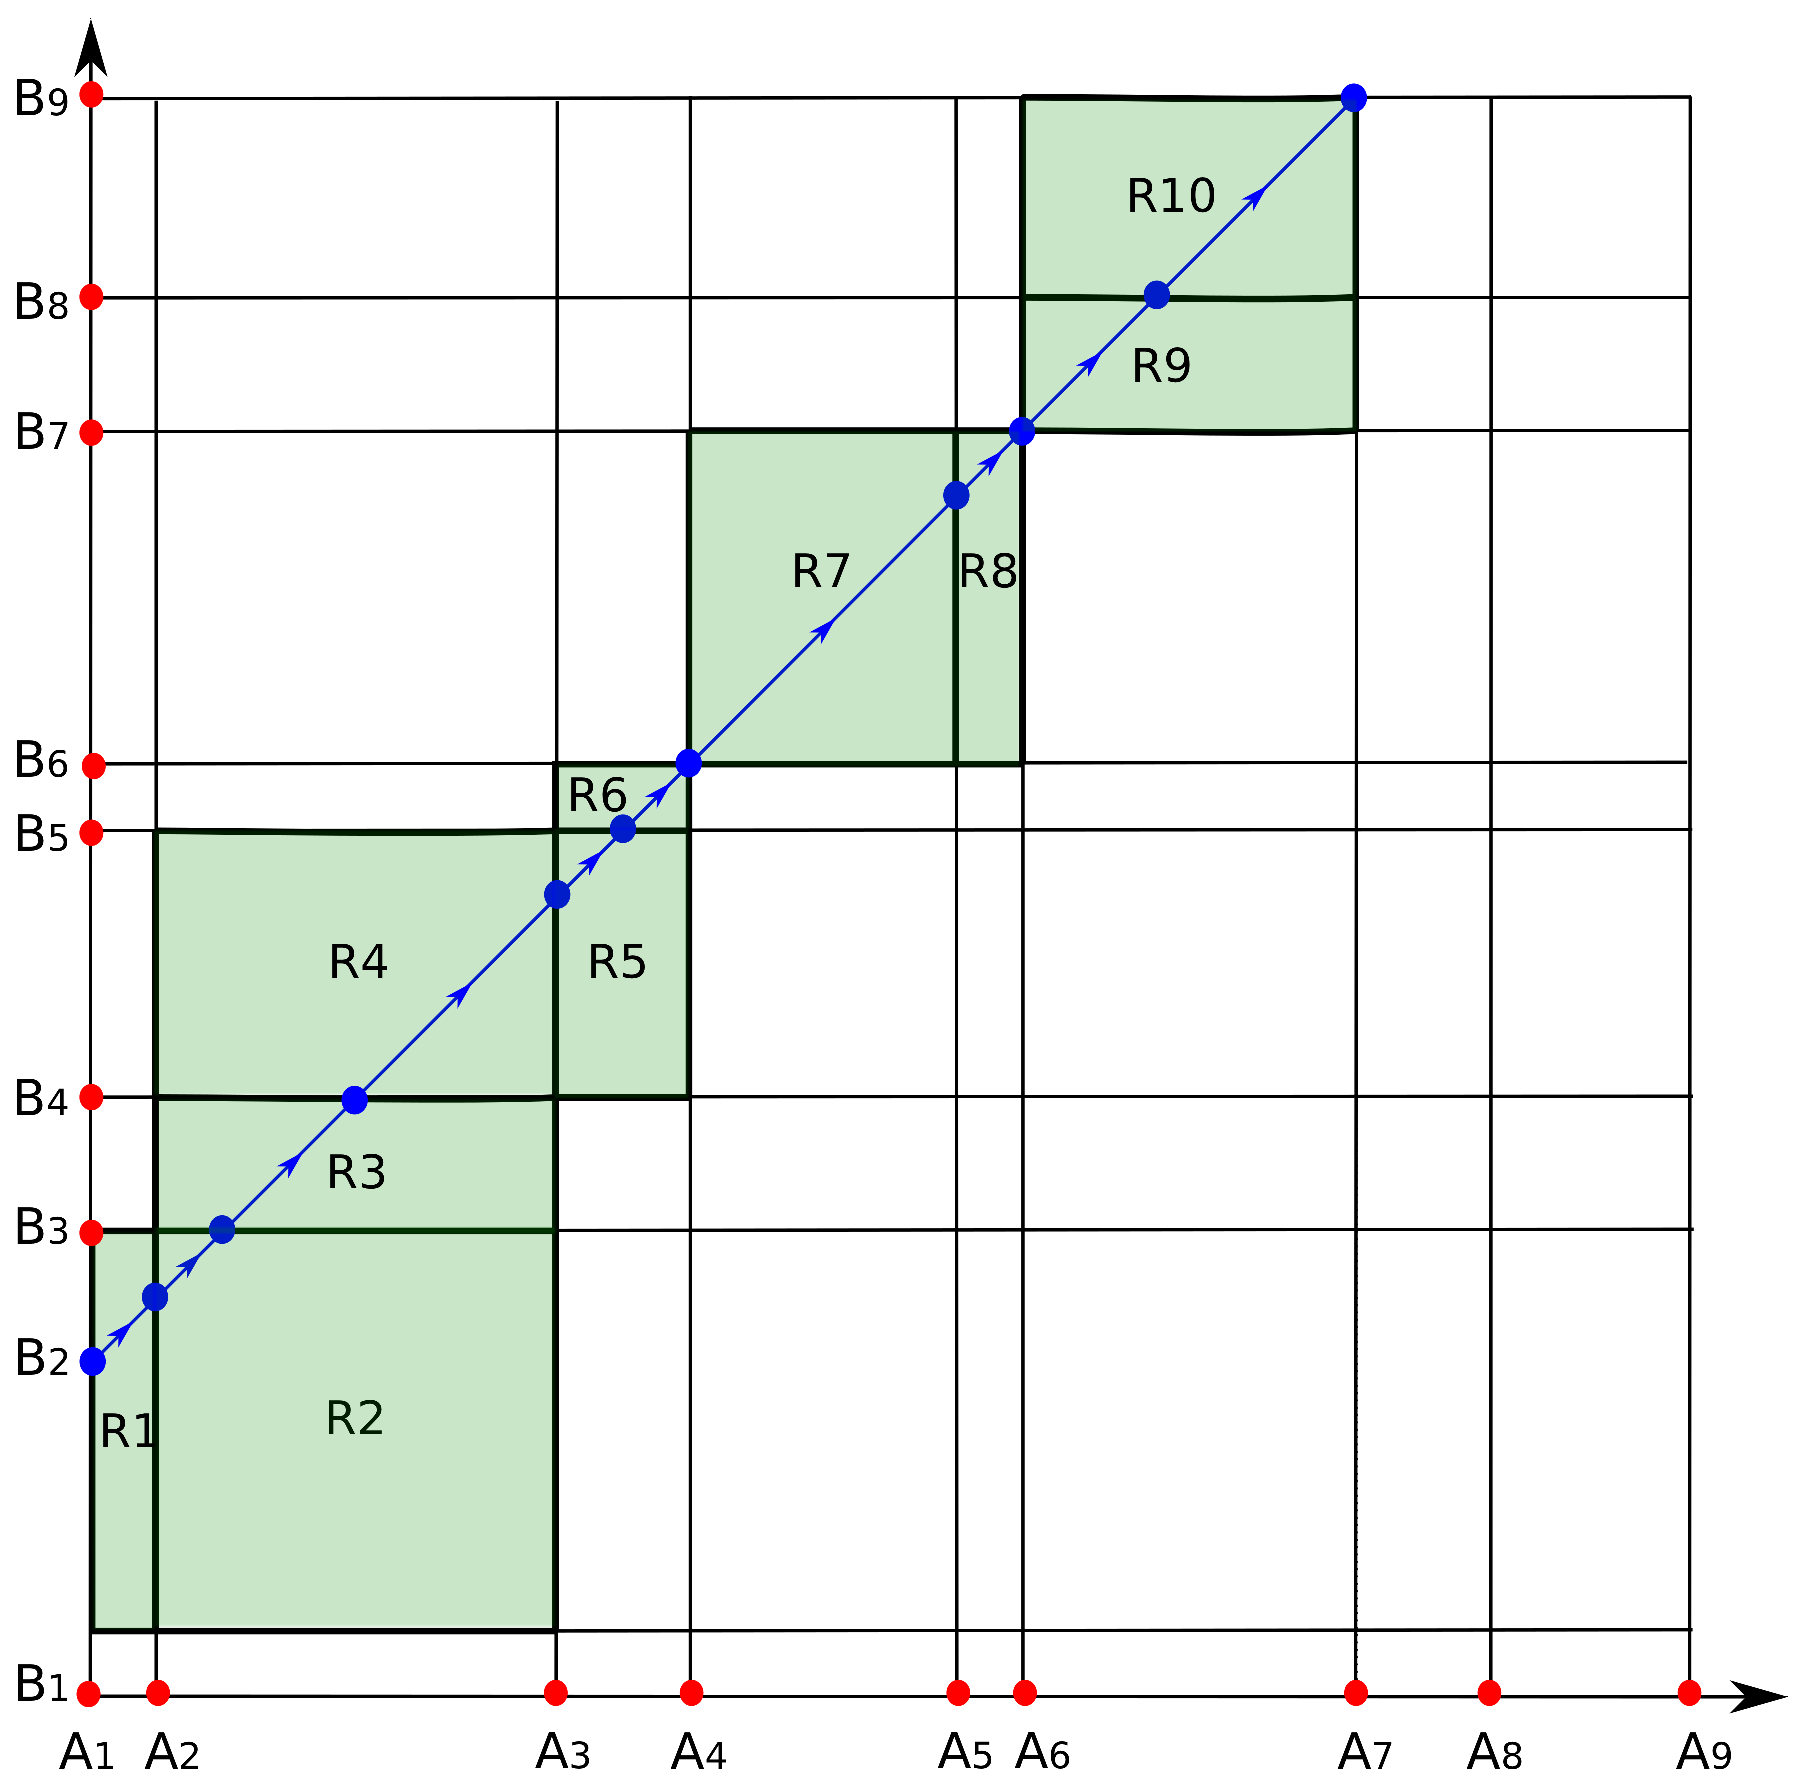
\includegraphics[scale=0.3]{fig/gridGraph.eps}
\caption{A sequence of $9$ points on the vertical axis and 9 points on the horizontal axis forms a grid with $(9-1) \times (9-1)$ rectangles.
The diagonal grid graph (consists of blue rectangles --- rectangles intersected by the blue line). }
\end{figure}


\subsection{From Genome Assembly Using Mate-Pairs to Rectangle Graph}

We represent presented genomes as circular strings over the alphabet of nucleotides: $\{A,T,C,G\}$. 
A $k$-mer is a string of length $k$.
Given a $k$-mer $s = s_1\ldots s_k$,
we define $prefix(s)= s_1\ldots s_{k-1}$ and $suffix(s) = s_2\ldots s_k$. Given a multi-set $A$ of $k$-mers generated from a genome, 
the standard de Bruijn graph has directed edge $(prefix(s) \rightarrow suffix(s))$
for each $k$-mer $s\in A$.  A vertex $v$  precedes (follows) vertex $w$ if there exists an edge from $v$ to $w$ (from $w$ to $v$). The in degree (out degree)  of a vertex 
$v$ is the number of vertices preceding (following) it.  A vertex $v$ is called a branching vertex if either its in degree or out degree is larger than 1. A path a $G$ is called a non-branching path if all of its vertices (but not the first and last) have indegree and outdegree
both equal to 1. %These non-branching path represents contigs in the fragment assembly problem.


\noindent
\textbf{A 2D coordinate of the genome}
Alternatively, the genome $S$ can also be represented as a sequence of $(k-1)$-mers $a_1\ldots a_n$ where 
$a_i$ corresponds to a $k-1$-mer starting at position $i$ on the genome. 
Each element of $S$ also corresponds to a vertex in the de Bruijn graph $G$. 
Let $t$ be the number of elements in $S$ that correspond to the branching vertices in the
de Bruijn graph. Element of $S$ that correspond to branching vertices in $G$ are called branching element. 
The substring $a_i, \ldots a_j$ of $S$ limitted by two consecutive branching 
elements $a_i$ and $a_j$ corresponds to a non-branching path in the de Bruijn graph; we call 
$a_i\ldots a_j$ a non-branching substring of $S$.

We now form a 2D coordinate of the genome by representing the genome $S=a1\ldots a_n$ on
both vertical and horizontal axis. $t$ branching elements 
in $S$ are colored in red in each axis. These points on both axis defines a grid, 
comprising of $t\times t$ rectangles. Each rectangle in this grid is defined by two adjacient branching 
elements in vertical and two adjacient branching elements in horizontal axis. 
Or equivalently, it is defined by a pair of (directed) non-branching substrings of $S$.    
In this coordinate, each point is labeled by a pair of $(k-1)$-mers. An edge of a rectangle is labeled 
by a list of all of its points.  

\noindent
\textbf{Mate-pairs and Diagonal Grid Graph}

Given a parameter $d$, a pair of $k$-mers $x$, $y$ forms a $(k,d)$-mer $(x|y)$  % here you say that two (k-1)-mers form (k,d)-mer (without -1), but the lext line uses (k-1,d)-mer.
of the genome $S = a_1\ldots a_n$ if there exists position $i$ such that $x=a_i$ and 
$y = a_{i+d}$ in $S$. The set of all $(k-1,d)$-mers of $S$ corresponds to a line $(d): y = x+d$.
% no! corresponds to a main diagonal $y = x$, not +d. Diagonal $y = x + d$ is for (x|x) (always happens in rectangles with equal sides, i.e. with distance zero between sides)
The line $(d)$ defines the \emph{diagonal grid graph} by retaining only the rectangles that 
are intersected by $(d)$. 

Below, we characterize the properties of the rectangles that are intersected by $(d)$. 
Since each rectangle $R$ is formed by a pair of non-branching substrings $\alpha = a_i\ldots a_{i+t1}$
and $\beta = a_i^*\ldots a_{i^*i+ t2}$, it is intersected by the line $(d)$ if and only if 
there exists $x$ such that $i\leq x \leq i+t1$ and $ i^* \leq x + d \leq i^* + t2$ (1). This condition
immediately leads to a property that there exists a $(k-1,d)$-mer $(a|b)$ of $S$ such that 
$a$ \emph{belongs} to $\alpha$ and $b$ \emph{belongs} to $\beta$.  A pair 
of non-branching substrings $\alpha$ and $\beta$ is called $d$-bounded if it corresponds to 
a rectangle intersected by $(d)$. The position where the (d) enters the rectangle is $(x^*,x^*+d)$ where 
$x^*$ is the minimum value  of $x$ such that condition (1) satisfies, and is labeled by 
a pair of $(k-1)$-mers $(a_{x^*}, a_{x^*+d})$.  The position where (d) exists 
the rectangle is $(\hat{x}, \hat{x}+d)$ where $\hat{x}$ is the maximum value of $x$ such that the condition
(1) satisfies, and this position is labeled by a pair of $(k-1)$-mers $(a_{\hat{x}}, a_{\hat{x} +d})$.


Given a $d$-bounded rectangle $R$ formed by a pair of non-branching substrings $\alpha = a_i\ldots a_{i+t1}$
and $\beta = a_i^*\ldots a_{i^*i+ t2}$, let $D_R= i^* - i$ be the genomic distance between $\alpha$ and $\beta$. The integer 
coordinate of the start $S(R)$ of the rectangle is $(i, i + D_R)$. By translating the origin from  $O$ to $S(R)$ for the line
$(d): y = x + d$, we obtain $(d'): Y = X + d - D_R$: the function of the line in a new coordinate: rectangle $R$. Given a fixed
value of $d$, the position of the line in each rectangle depends on $D_R$. In other words, the line on each rectangle $R$ 
uniquely defines the genomic distance between $\alpha$ and $\beta$ and vise versa. 


\noindent
\textbf{From mate-pair assembly with exact distance to the rectangle Graph}
While the line $(d)$ represents the 
set of points in the $2D$ coordinate (coordinate of pairs of $k$-mers), it uniquely defines the genome.
In the fragment assembly problem from a from a set of all $(k,d)$-mers of the genome, 
the diagonal grid graph is unknown, but each separated rectangle as well 
as the line segment on it can also be generated
from the set of $(k,d)$-mers. The task of assemblying the genome from mate-paired reads can be 
reduced to the problem of reconstructing the diagonal line --- which implies solving the simplified jigsaw problem from separated rectangles. Below we describe how
to generate rectangles and line segments on these rectangles from a set of all $(k,d)$-mers of an unknown genome. We now 
show that all d-bounded rectangles as well as the position of the line fragment on each of these rectangles can be constructed from 
the set of $(k,d)$-mers. 


%    We now show that every d-bounded rectangle formed
%    by a pair of non-branching substrings $\alpha = a_i\ldots a_{i+t1}$ and $\beta = a_j\ldots a_{j+t2}$, 
%    we can construct a rectangle having the same labels of the edges as well as the position of the line fragment on it from only 
%    a set $A$ of all $(k,d)$-mers of the genome. 



Let $G$ be the de Bruijn graph constructed from a set of 
$k$-mers in $A$. A pair of non-branching paths $p_1$, $p_2$ is called $d$-bounded if there is a $(k,d)$-mer $(a,b)$ such that 
$a$ maps to $p_1$ at position $i_1$ and $b$ maps to $p_2$ at position $i_2$. The genomic distance between the starts 
of $p_1$ and $p_2$ is $D = d + i_1 - i_2$. A trible $(p_1, p_2, D)$ corresponds to a set of pairs of non-branching substrings 
$\{\alpha, \beta\}$ in the genomes where $\alpha$ ($\beta$) has same label as $p_1$ ($p_2$)  and their genomic distance between them 
is $D$. Thus, as mentioned above, it uniquely defines a rectangle as well as the line fragment on it. Thus, from a set of $(k,d)$-mers, 
 we can construct a set of all d-bounded rectangle as well as the position of the line fragments on it. 
The questions of reconstructing the line ( and thus, reconstruct the sequence) is now reduced to the jigsaw puzzle. We simply construct the 
rectangle graph based on the described procedure. Moreover, the property that in the de Bruijn graph there is a single vertices for each $k$-mers simplifies
the presentation of the rectangle graph. In fact, a single pair of $k$-mers can uniquely identify the edge of a rectangle. Below we describe 
the \textbf{rectangle algorithm} for genome assembly from a set of $(k,d)$-mers of the genome.   


\noindent
\textbf{Rectangle Graphs for a set of $(k,d)$-mers}
\bigskip
\begin{algorithmic}[1]
\REQUIRE Set of $(k,d)$-mers 
\STATE Construct the  de Bruijn graph from individual  $k$-mers.
%\STATE Construct the   de Bruijn graph
\STATE Transform the set of $(k,d)$-mers into the set of rectangle triples. 
\STATE Represent each rectangle triple as a rectangle with a line segment.
\STATE Represent the rectangle as an edge: $u\rightarrow v$.
\STATE \hspace*{0.5cm} $u$ is labeled by a pair of $k$-mers corresponding to the begin of the line.
\STATE \hspace*{0.5cm} $v$ is labeled by a pair of $k$-mers corresponding to the end of the line.
\STATE Construct the rectangle graph by gluing vertices having the same label together.
\STATE Output contigs from non-branching paths in the rectangle graph.
\end{algorithmic}

\noindent
\textbf{From mate-pair assembly with inexact distance to the rectangle Graph}

We now extending the rectangle graphs to model genome assembly problem from mate pairs when the distance 
between two reads in each pair is not exact. Given parameters $d$ and $\Delta$, 
a pair of $k$-mers $(a|b)$ is called a $(k,d,\Delta)$-mer of $S$
if it is a $(k,d_0)$-mer of $S$ for some $d_0 \in [d-\Delta, d+ \Delta]$. While the set of all $(k,d)$-mer 
of $S$ forms a line $(d) y = x + d$ in the 2D genome coordinate, a set of $(k,d,\Delta)$-mers forms 
separated points perturbed around $(d)$. And thus, in each rectangle, the line fragment now becomes a collection of points 
perturbed around its original position.
The task of assemblying the diagonal grid graph from inexact mate pairs is analogous to 
the solving the old jigzaw problems where the pictures on each pieces are faded out, some pieces from other puzzles got mixed into 
the collection, or even some of the pieces are missing. Bellow we address these complications.

\noindent 
\textbf{Line Fragments Reconstruction} 
We now describe how to reconstruct the line fragment on each rectangles from a collection of perturbed points corresponding to the 
inexact $(k,d,\Delta)$ mers.  


 To better \emph{repaint}
the line segment, it is beneficial to first characterize the variation of insert size. 

While it is commonly accepted that insert size distribution for multiple cell data follows a Gaussian distribution,
in single cell dataset the insert size distributions are often skewed. Fortunately, it is often the case 
that the distribution is unimodal and we exploit this property to make our line fragments reconstruction procedure work well for
both single cell and multiple cell dataset. We initially obtain the empirical distribution of the insert size 
by mapping read pairs to long edges in the graph. We set $d$ equal to the mode of the distribution.  



A pair of condensed path $p_1$ and $p_2$ in the graph is called a d-bound suspected if there exists 
a pair of $(k,d)$-mers $(a,b)$ such that $a \in p_1$ and $b\in p_2$. For each d-bounded suspected pair of condensed paths, we draw a rectangle with
vertical edges $p_1$ and horizontal edges $p_2$. For each pair of $k$-mers $(a,b)$, we draw a point $(x,y)$  on the rectangle 
where $x$ is the position on the horizontal edge corresponding to $k$-mer $a$ and $y$ is the position on the vertical edge 
corresponding to $k$-mer $b$. The position of these points on the rectangle approximate the genomic  distances between $p_1$ 
and $p_2$. Since the genome is an edge-covering tour in the de Bruijn graph,  the genomic distances between $p_1$ and $p_2$ corresponds to
the lengths of some paths connecting $p_1$ and $p_2$. Let ${\ell_1, \ldots \ell_t}$~\footnote{ If $t = 0$ (there is no path
connecting $p_1$ and $p_2$ within the distance constraint), we remove this rectangle from further analysis} be a set of all graph distance between 
$p_1$ and $p_2$ that are in the range of $[d - |p_1|, d]$.  We draw $t$ lines  $(d_i): y = x + d - \ell_i$ where $ 1 \leq i \leq t$.  Among 
 these $t$ lines, only $t' \leq t$ represent the fragment of the original line on the diagonal grid graph. In other words, 
    they corresponds to the genomic distances between $p_1$ and $p_2$. 
 Our goal is to identify 
these $t_1$ lines among $t$ possible lines, which are now represented as perturbed points on the rectangle.


Since $d$ was chosen at the median of the distribution, the points corresponding to a line $(d_i)$ will be more probable 
to perturbate closer to the line than farther from it. For each line we define a supporting value $v_{sp}$, which is the weighted density of 
points in the $\epsilon$ distance around it: $v_{sp} = \sum_{(x_j,y_j)}\frac{ \mathbf{f}(y_j - (x + d - \ell_i) ) I((x,y), \epsilon) }{length(d_i)}$, where
$\mathbf{f}$ is the empirical probability densitry function of the insert size; $I((x_j,y_j), \epsilon)$ 
is the identicator function that indicates whether a point $(x_j,y_j)$
lies in the region defined by $d - \ell_i - \epsilon$ and $y = x + d - \ell_i + \epsilon$


We empirically choose a threshold and ignore all lines that have the supporing values smaller than the threshold. The weakness of this approach is that 
if two lines $(d_i)$ and $(d_j)$ are close, a majority of points that supports line $d_i$ will also supports line $d_j$ and vise versa.  
This leads to the problem of selecting the incorrect line fragments around the correct ones. To overcome this problem, for a pair of 
lines $(d_i)$, $(d_j)$, we define a separating value equal to the minimum supporting value of any line drawing between $(d_i)$ and $(d_j)$.
Note that the separation values usually use smaller $\epsilon$ than  the supporting values.  The separating values further divide the 
list of remaining lines into partitions, each partition represents single lines or consecutive lines that can not be separated. We 
represent each partition on each rectangle. 

\noindent
\textbf{Rectangle Graph for Approximate Distance}
As mentioned above, the variation of the distance of insert size transform the line fragment on each rectangle into a set of
perturbed points around it. While the \emph{Line Fragments Reconstruction} procedure described above attemps to reconstruct the line, it can not guarantee 
to have a single line on each rectangle but instead, can result in multiple (parallel) lines closed to each other, where we can guarantee that at least 
one of them is the correct line fragment of the original line. Thus, the extending condition for rectangles should be revised so that the original line can be
reconstructed by extending the rectangles.  

We represent the incoming/ outgoing face of a rectangle as  a set of pairs of $k$-mers, corresponding to the starts/ends of the lines in the rectangle. 
Rectangle $R_1$ can extends rectangle $R_2$ ($R_2$ is extendable by $R_1$) if the outgoing face of $R_2$ shares at least 
one pair of $k$-mers with the incoming face of $R_1$.  The lines in $R2$ corresponding to the shared pair of $k$-mers are called extendable lines with respect to
$R_1$. If a line is not extendable by any other rectangle, we remove it from the rectangle.  Additionally, if a rectangle $R_2$ have $r$ lines and each line 
is extendable by $r$ different rectangles that can not extend any other rectangle except for $R_2$, we replace $R_2$ by $r$ different rectangles, each with 
a single line. 
 
Finally, the rectangle graph is constructed by: (1) Represent each rectangle as an edge from its in-coming 
face to its out-going face; (2) Glue two node if they share at least one pair of $k$-mer. We output contigs from non-branching path in the rectangle graph. 


\begin{figure}
\begin{center}
	\begin{tabular}{l@{\extracolsep{13pt}}l}
		(a) & (b) \\
		\vtop{\vskip0pt\hbox to.45\textwidth{\includegraphics[width=.45\textwidth] {fig/ecolilane1.eps}}}
		&
		\vtop{\vskip0pt\hbox to.45\textwidth{\includegraphics[width=.45\textwidth] {fig/saureuslane7.eps}}}
	\end{tabular}
    \caption{Distribution of insert size for Single Cell Datasets of \emph{E.coli} and \emph{S. aureus}}
    \label{fig:distri}
\end{center}
\end{figure}

\begin{figure}
\begin{center}
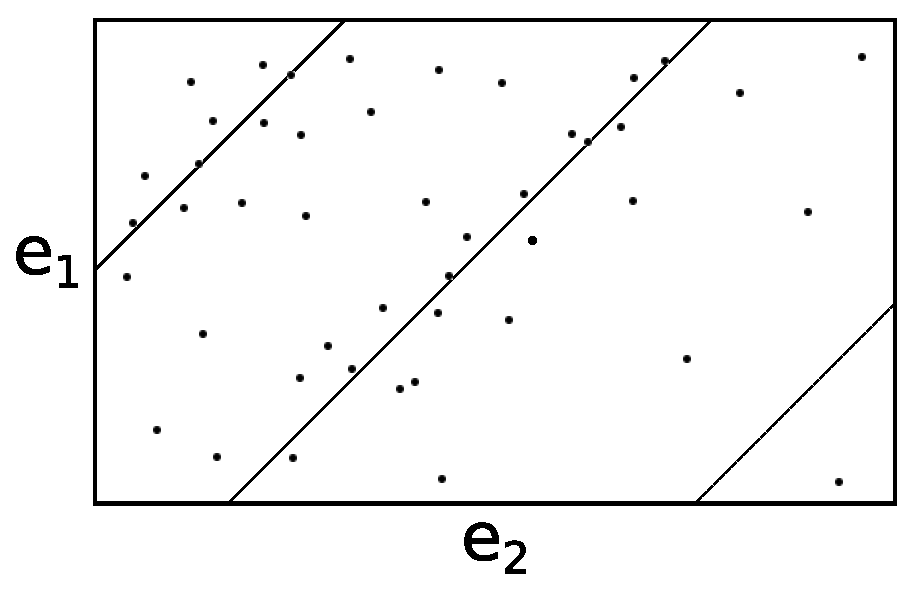
\includegraphics[scale=0.5]{fig/rectangle.eps}
\caption{Example of rectangle with three diagonals. Rightmost diagonal isn't well supported mate pairs, 
while other two are well supported. The point which is observed in the lower right corner 
could appear because of chimeric mate pairs or sequencing errors.}
\end{center}
\end{figure}

\noindent
\textbf{Recovering Missing Rectangles}

Because of the variation in the insert size, some d-bounded pair of paths $(p_i,p_j)$ may have no mapping pair 
of reads~\footnote{Especially when these paths are short} (pair of reads that connect these two paths). 
This leads to the problem of missing some rectangles in the rectangular
puzzle. Fortunately, similar cases also happen in the ordinary jigsaw puzzle.
Old jigsaw puzzles sometimes also lose some pieces. A common approach is assembling with the remaining pieces first and later, verifying  
the solution by checking if the holes in the resulting figure can actually be fit by any common jigsaw pieces. A more miticulous 
player after assemblying the figure, may make new pieces that match the holes and try to draw on the new parts to make a complete picture. 
We borrow this approach for recovering missing rectangles. Before describing the algorithm, we first define some notions.

Given two rectangles $R_1$ and $R_2$: $R_1$  with sink $(a_1|b_1)$  and $R_2$ with source  $(a_2|b_2)$ (we remind 
that sink/source of a rectangle is labeled by a pair of $k$-mers corresponding to the start/end point of the line segment in the rectangle).  
$R_1$ and $R_2$ are \emph{linkable} if there exist two paths of equal length $p(a_1, a_2): a_1 \leadsto a_2$ and $p(b_1, b_2): b_1 \leadsto b_2$
in the de Bruijn graph, and the minimum length of such paths is called the distance between $R_1$ and $R_2$. 
Given the rectangle graph constructed from a set of rectangles,  a rectangle is called a sink~\footnote{The sink of the rectangle graph is a rectangle, the sink of 
a rectangle is the the side that the line segment enters the rectangle (represented as a pair of $k$-mers).} if its source is not connected 
to any other rectangle. Similarly, a rectangle is called a source if its sink is not connected to any other rectangle. Below we describe a 
procedure that heuristially recovering missing rectangles. 

Let $SOURCE$ be a set of sources rectangles and $SINK$ be a set of sinks rectangles in the rectangle graph. 
For a rectangle $R_i \in SINK$, we choose a rectangle $R_j \in SOURCE$ such that the distance from $R_i$ to $R_j$ is minimum.
 We form a new rectangle $R_{i+1}$ 
such that: (i) the source of $R_{i}$ can only be connected to the sink of $R_{i+1}$, (ii)  distance from $(R_{i+1})$ to $R_{j}$ is smaller than
the distance from $R_i$ to $R_j$, (iii) $R_{i+1}$ either connects to $R_j$ or becomes a sink nodes in the new rectangle graphs. If $R_{i+1}$ is not
connected to $R_j$, we continue to extend $R_{i+1}$ in the same way.  The procedure is succefull if at each step, only a unique rectangle  $R_{i+1}$ 
can be constructed and the total length of all line segments in the added rectangles does not exceed a certain threshold. 
If the procedure is not succesful, we backtrack and undo all the changes that attempt to connect $R_i$ to $R_j$.

We now show how to construct a new rectangle that can connect to a rectangle...
NOT YET FINISHED.
\section{Results}

\textbf{Assembly Datasets}
We used three datasets from \cite{Chitsaz2011}.
A single {\ecoli} cell
and a single marine cell ({\em Deltaproteobacterum} SAR324)
were isolated by micromanipulation as described in \cite{Ishoey2008}.
Paired-end libraries were generated on an Illumina Genome Analyzer IIx from MDA-amplified single-cell DNA
and from standard (multicell) genomic DNA prepared from cultured {\ecoli}.

We call these datasets SAR324, ECOLI-SC, and ECOLI-MC.
ECOLI-SC and ECOLI-MC are called ``{\ecoli} lane 1'' and ``{\ecoli} lane normal'' in \cite{Chitsaz2011}.
They consist of 100 bp paired-end reads
with average insert sizes 266 bp for ECOLI-SC, 215 bp for ECOLI-MC,
and 240 bp for SAR324.
All datasets have $600\times$ coverage.

\textbf{Benchmarking}

We benchmarked seven assemblers
(EULER-SR \cite{Chaisson08}, IDBA \cite{Peng10}, SOAPdenovo \cite{Li10}, Velvet \cite{Zerbino08}, Velvet-SC \cite{Chitsaz2011}, E+V-SC \cite{Chitsaz2011} and {\spades}) on three datasets
(ECOLI-SC, ECOLI-MC, and SAR324). To provide unbiased
benchmarking, we used the assembly evaluation tool Plantagora \cite{Barthelson2011}. See Table \ref{Table1}.

{\spades}-rectangle shows improvement over previous SPAdes algorithms. In ECOLI-MC dataset {\spades}-rectangle produce larger N50, almost the same largest contig and the same number of misasseblies.

Improvement is even more significant for single-cell dataset which can be explained by the fact that {\spades}-rectangle better determine and utilize correct distance between edges in the de Bruin graph given datasets with highly uneven coverage. {\spades}-rectangle procudes higher N50 (56,842 bp vs 49,623 by {\spades}), higher largest contig (209,690 bp vs 177,944 by {\spades}), no misassemblies and also captures 64 additional genes (3975 vs 3911 by {\spades}). All other assemblers except of {\spades} and {\spades}-rectangle produced below average results on the single-cell dataset.

Most important that on all datasets {\spades}-rectangle was able to capture more genes than any previous assemblers including {\spades}. New genes are most important in study of new species that cannot be sequenced by classical multi-cell approach.

We further compared E+V-SC, {\spades} and {\spades}-rectangle on the SAR324 dataset.
{\spades}-rectangle assembled contigs totaling ????? bp
(vs. 5,129,304 bp for {\spades} and 4,255,983 bp for E+V-SC) and an N50 of ????? bp (as compared to 75,366 bp for {\spades} and 30,293 bp for E+V-SC).
Since the complete genome of \emph{Deltaproteobacterium} SAR324 is unknown,
we used {\em long ORFs} to estimate the number of genes longer than 600 bp, as a proxy for assembly quality (see \cite{Chitsaz2011}).
There are ???? long ORFs in the {\spades}-rectangle assembly
vs. 2603 for {\spades} and 2377 for E+V-SC.
% I forgot to run on SAR324, doing it now.

%\def\ra#1{\rotatebox{90}{\parbox{1.0in}{#1}}}
\def\mrk#1{{\bf #1}}


%%%%%%%%%%%%%%%%%%%%%%%%%%%%%%%%%%%%%%%%%%%%%%%%%%
% Table notes, adapted from PNAS
\newcount\tablenoteloopnum
\newcount\tablenotenum

\makeatletter
\def\tablenote#1{\global\advance\tablenotenum by 1\relax
$^{\@alph{\the\tablenotenum}}$\expandafter\gdef\csname 
tabnote\the\tablenotenum\endcsname{#1}}

\def\tablenotes{\tablenoteloopnum=\tablenotenum
\global\advance\tablenoteloopnum by 1
\tablenotenum=0
{\footnotesize
\leftskip=0pt \rightskip=\leftskip
\parfillskip=0pt plus 1 fil
\loop
\vskip2pt
\noindent
\global\advance\tablenotenum by 1
\ifnum\tablenotenum<\tablenoteloopnum
$^{\@alph{\the\tablenotenum}}$\csname 
tabnote\the\tablenotenum\endcsname
\repeat}
}
\makeatother
%%%%%%%%%%%%%%%%%%%%%%%%%%%%%%%%%%%%%%%%%%%%%%%%%%

\begin{table}
\small

\caption{
%\textbf{Table~1.
Comparison of assemblies
for
single-cell (ECOLI-SC) and
standard
(ECOLI-MC) datasets.
}\label{Table1}


%\vspace*{-0.2in}

\tabcolsep=4pt
%\rowcolors{1}{}{lightgray}
\begin{tabular}{@{\extracolsep{1pt}}p{.2in}p{1.1in}rrrrrrrr}
%\begin{tabular*}{\hsize}{@{\extracolsep{\fill}}p{.2in}p{1.1in}rrrrrrrr}
%\begin{tabular}{p{.2in}p{1.1in}rrrrrrrrr}
%\toprule
 &
    Assembler%
    \tablenote{%
      The best assembler by each criteria is
      indicated in bold. EULER-SR 2.0.1, Velvet 0.7.60, Velvet-SC, and
      E+V-SC were run with vertex size 55.
      %equal to 55.
      %Edena 2.1.1 49 was run with a minimum overlap of 55.
      SOAPdenovo 1.0.4 was run
      with vertex size 27--31. IDBA was run in its default iterative mode;
      IDBA crashed on ECOLI-SC, so IDBA results are only shown for ECOLI-MC.
      {\spades}-single refers to {\spades} without Stages 2 and 3,
      %(without using read-pair information)
      for
%       an unbiased 
       comparison with E+V-SC, which does not use read-pair information.
      {\spades}, {\spades}-single and {\spades}-rectangle iterated over 
      %vertex sizes 21, 33, 55 (
      edge sizes $k=22,34,56$.
      %{\ecoli} gene annotations
      %were from http://www.ecogene.org/\;.
       Statistics in this table differ slightly from statistics presented in~\cite{Chitsaz2011}
       due to the specific criteria used in Plantagora.
     %  \glenn{Alexey et al: It's not just the number of misassemblies that changed.  Also substitution error rate changed (why?) and number of complete and partial genes changed.  Are you using the same set of annotated genes that I gave you that were used in the Chitsaz et al paper, or a different set?  Do you show all contigs, or do you filter out contigs below a certain size (110 bp was used in Chitsaz et al, 200 bp is used in HMP consortium).  Please at least explain it by email; we need to be prepared to explain this discrepancy if a referee asks.}
%       since Plantagora has a strict criteria for misassemblies.
      % \glenn{There are differences in substitution error rate and numbers of complete and partial genes as well.  Is the SP lab using a different set of annotated genes?  Different small contig size cutoff?  Etc.  We have to change this explanation.}
    }
 & \# contigs
 & N50~(bp)
 & Largest~(bp)%
  \tablenote{Length of the largest contig without a misassembly.}
 & Total~(bp)%
        \tablenote{The total assembly size may increase (and in some cases exceeds the
         genome size) due to contaminants (see~\cite{Chitsaz2011}),
         misassembled contigs, repeats, and hubs that contribute to multiple contigs.
         The percentage of the {\ecoli} genome covered filters out these issues.
         %Since our datasets include contaminant reads (see~\cite{Chitsaz2011}),
         % for details),
         %the total assembly size may exceed the genome size.
        }
 & Covered (\%)%
       \tablenote{\emph{Percent of genome covered} is the ratio of total number of aligned bases in the assembly to the genome size.
       %This may shrink from the total assembly size due to assembly of contaminants.
%       However, it may also increase due to small contigs that align to multiple places.
%       (which are counted with multiplicity by Nucmer).
%       Note that some small contigs may align to multiple places in the genome, and thus
%       increase the percent of genome covered.
     %  \glenn{Alexey needs to add a brief description earlier of how we used Plantagora, MAUVE, and Nucmer, and citations for all three, not just Plantagora.}
       }
 & MA%Misassemblies%
       \tablenote{MA: \emph{Misassemblies} are locations on an assembled contig where the left flanking sequence aligns over 1~kb away from the right flanking sequence on the reference.}
 & MM%Mismatches (per 100 kbp)%
       \tablenote{MM: Mismatch (substitution) error rate per 100 kbp is measured in the correctly assembled contigs.}
 & CG%Complete genes%\\
       \tablenote{CG: Complete genes out of 4,324 genes annotated at http://www.ecogene.org\;.}
 %(among 4324 known)
% & \ra{Complete plus \\ partial genes%
%       \tablenote{
%         ``Partial genes'' are genes with an overlap of at least 100 nucleotides
%         with a contig, but not wholly contained in the contig;
%         see~\cite{Chitsaz2011}.
         %``Partial genes'' are defined as in~\cite{Chitsaz2011}.
         %A gene is ``partially'' present in the assembly if it has an overlap
         %of at least 100 nucleotides with a contig, but is not completely
         %contained in the contig.
%       }
%   }
 \\
   \hline
%\midrule
%\smallskip
\\[-6pt]
\multicolumn{10}{l}{\bf Single-cell {\ecoli} (ECOLI-SC)}\\
%\\[-9pt]
 & EULER-SR                 &      1344 &           26662 &                       126616 &    4369634 &         87.8 &            21 &                     11.0 &                   3457 \\%&         3889 \\
%& Edena                    &      1592 &            3919 &                        44031 &    3996911 &         79.1 &            12 &                      2.1 &                   2440 &         3569 \\
 & SOAPdenovo               &      1240 &           18468 &                        87533 &    4237595 &         82.5 &            13 &                     99.5 &                   3059 \\%&         3653 \\
 & Velvet                   & \mrk{428} &           22648 &                       132865 &    3533351 &         75.8 &             2 &                \mrk{1.9} &                   3117 \\%&         3288 \\
 & Velvet-SC                &       872 &           19791 &                       121367 &    4589603 &         93.8 &             2 &                      \mrk{1.9} &                   3654 \\%&         4010 \\
 & E+V-SC                     &       501 &           32051 &                       132865 &    4570583 &         93.8 &             2 &                      6.7 &                   3809 \\%&         4001 \\
  & {\spades}-single               &      1164 &           42492 &                       166117 &    4781576 &   \mrk{96.1}  &       1 &                      6.2 &                   3888 \\%&   \mrk{4177} \\
 & {\spades}                   &      1024 &     49623 &                 177944 &    4790509 &         \mrk{96.1} &       1 &                      5.2 &             3911 \\ %&         4172 \\[3pt]
 & {\spades}-rectangle                   &      509 &     \mrk{56842} &                 \mrk{209690} &    4550761 &         95.5 &       \mrk{0} &                      3.6 &             \mrk{3975} \\[9pt] %&         4172 \\[3pt]
 %
%
% & {\spades}-single reads               &      1241 &           38138 &                       133927 &    4621694 &   \mrk{96.12}%
%\tablenote{A manual analysis revealed that a  212 bp contig marked as misassembled by {\spades}-single is actually a Plantagora alignment artifact.
%% rather than misasembly.
%}
%  &             1 &                      3.3 &                   3879 &   \mrk{4179} \\
% & {\spades}                   &       845 &     \mrk{45436} &                 \mrk{209370} &    4633764 &         95.65 &       \mrk{0} &                      5.5 &             \mrk{3892} &         4158 \\[3pt]
\multicolumn{10}{l}{\bf Normal multicell sample of {\ecoli} (ECOLI-MC)}\\
%\\[-9pt]
 & EULER-SR                           &       295 &    \mrk{110153} &            221409 &    4598020 &        99.5 &            10 &                      5.2 &                  4232 \\%&         4306 \\
%& Edena                              &      1673 &            3814 &             20470 &    4611645 &        97.0 &             6 &                      2.8 &                  3020 &         4212 \\
& IDBA                               & \mrk{191} &           50818 &            164392 &    4566786 &        99.5 &             4 &                      1.0 &                  4201 \\%&         4314 \\
 & SOAPdenovo                         &       192 &           62512 &            172567 &    4529677 &        97.7 &             1 &                     26.1 &                  4141 \\%&         4220 \\
 & Velvet                             &       198 &           78602 &      196677 &    4570131 &       \mrk{99.9} &             4 &                1.2 &                  4223 \\%&         4309 \\
 & Velvet-SC                          &       350 &           52522 &            166115 &    4571760 &        \mrk{99.9} &       \mrk{0} &                      1.3 &                  4165 \\%&         4265 \\
 & E+V-SC                             &       339 &           54856 &            166115 &    4571406 &        \mrk{99.9} &       \mrk{0} &                      2.9 &                  4172 \\%&         4264 \\
 & {\spades}-single                         &       445 &           59666 &            166117 &    4578486 & \mrk{99.9} &       \mrk{0} &                     \mrk{0.7} &                  4246 \\%&   \mrk{4317} \\
 & {\spades}                             &       195 &           86590 &            \mrk{222950} &    4608505  &   \mrk{99.9}  &             2 &                      3.7 &             4268 \\%&    \mrk{4318} \\
 & {\spades}-rectangle                   &      192 &     91893 &                 221829 &    4593658 &         \mrk{99.9} &       2 &                      3.5 &             \mrk{4274} \\ %&         
 \hline
%\bottomrule
\end{tabular}

\bigskip

\tablenotes

%\bigskip


%\vspace*{-0.2in}

\end{table}


\textbf{Running time and memory requirements}

SPAdes memory and time complexity were analysed in \cite{SPAdes}. Most time and memory consuming stages in genome assembly are, usually, de Bruijn graph construction and mapping reads to edges. After this stages are done, repeat resolution routine can work relatively fast and within small memory.

For both {\ecoli} datasets and SAR324, our rectangle approach works for less then 10 seconds given (1) unresolved de Bruijn graph from SPAdes-single and (2) mapping positions of all mate-pair reads to the graph. All datasets where analysed using less than 100 MB RAM.

%\section{Basics}
%%
%\section{What is Diagonal}
%
%Define \textbf{point} in rectangle $(a|b)$ as ordered pair of $K$-mers in this edges $(a_i|b_j)$.
%
%Define \textbf{d-point} as point $(a_i|b_j)$ s.t. distance between $a_i$ and $b_j$ in genome is $d$. The goal is to use all d-points and only, but we don't know the truth...
%
%Two points are equal if their pairs of $K$-mers are equal.
%
%Define \textbf{diagonal} $(a|b, D)$ in rectangle $(a|b)$ with offset $D$ s.t. $-|b| \leq D \leq |a|$ as list of points $(a_i, b_{i-D})$ for $i = max(D, 0) ... min(|a|, |b|+D)$.
%
%Define \textbf{d-diagonal} as diagonal of only \textbf{d-points}. 
%
%Length of diagonal is number of points in this diagonal. E.g. diagonal $(a|a, d)$ have length of $|a| - d + 1$.
%
%Rectangles can contain multiple diagonals.
%
%\section{Diagonal Support}
%
%\textbf{Support} is our confidence that diagonal $(a|b, D)$ is actually d-diagonal.
%
%Diagonal $(a|a, d)$ for long enough edge $a: |a| \geq d$ is always d-diagonal and doesn't require any other support.
%
%Diagonal can be supported:
%\begin{enumerate}
%\item By points known to be d-points from the graph $G$, i.e. exists path of length $d$ (this initial support exists in all rectangles).
%\item By points known to be d-points from paired reads. TODO: use insert size variation. TODO: use PHRED-quality of particular K-mers.
%\item By points known to be d-points from single reads. E.g. if single read covers $a \rightarrow ... \rightarrow b$ connection and there exists rectangle $(a|b)$.
%\item TODO: PathSets?
%\item TODO: Neighbouring rectangles (diagonals) while gluing.
%\item TODO: Other diagonals in the same rectangle (how? see section Gluing).
%\end{enumerate}
%
%Support of diagonal should scale by the length of diagonal.
%
%\section{Rectangle Split}
%
%The main goal is to filter and split rectangles, so that each rectangle contain d-diagonal and it is the only diagonal in this rectangle.
%
%If one rectangle have multiple well-supported diagonals, we need to split it to multiple rectangles (one diagonal to each). Same applies for number of average-supported diagonals within variation (e.g. insert size variation), so their join is well-supported.
%
%\section{Do we need rectangles?}
%
%We can define everything only with diagonals, but it's simpler to draw them within rectangles.
%
%Rectangle is equal to set (cluster) of diagonals. Rectangles splitting is somewhat similar to the current distance estimation.
%
%\section{Diagonals Ranking}
%
%We sort diagonals by their support. Better supported goes first.
%
%\section{Diagonals Gluing}
%
%We glue diagonals by their end-points only if this end-points are equal.
%
%We glue diagonals in the order of their support:
%\begin{itemize}
%\item First we glue all well-supported diagonals (because they are d-diagonals).
%\item We iterate over average-supported diagonals in the order of their support:
%\begin{itemize}
%\item If diagonal can connect two hanging end-points of already used diagonals, we glue it (preferable).
%\item If diagonal can be glued to one hanging end-point of already used diagonal, we glue it.
%\end{itemize}
%\item We don't use poorly-supported diagonals.
%\end{itemize}
%
%\section{Gluing Support}
%
%Original gluing support (rule) is equality of glued end-points of diagonals.
%
%We can think about more gluing supports, e.g.:
%\begin{enumerate}
%\item Glue diagonals $(a|b, \cdot)$ and $(a|c, \cdot)$ only if there exists single read with $(K+2)$-mer which covers $b \rightarrow c$ path in graph. It's more powerful then single-read support for diagonals. TODO: $K+10$? $K+x$?
%\item PathSets were supposed to be one of gluing supports --- glue two diagonals only if first's pathset is a prefix of second's pathset. We can somehow use PathSets also in the diagonal support, but I don't know how :)
%\item TODO: more.
%\end{enumerate}
%

\bibliographystyle{plain}
\bibliography{mybib}

\end{document}
